\chapter{Segmentación con mascaras de color}
\label{chap:Segmentacion con mascaras de color}
\Abstract{El presente capítulo describe de forma detallada el proceso de análisis de imágenes mediante segmentación por color. El proceso para la detección de piezas se divide en tres fases: segmentación por color, mejora de la imagen y extracción de atributos.}

El primer paso para poder recolocar piezas es localizarlas. Con el objetivo de localizarlas, se han desarrollado múltiples herramientas capaces de hacerlo, pero cada una presenta grandes ventajas y desventajas. Pero para poder entender la evolución y el desarrollo de estas es necesario entender el contexto de este proyecto. Se parte del trabajo previo llevado a cabo por Ana Berjón \citep{TFGAna}, y el objetivo de este proyecto era el perfeccionamiento de este sistema. Tanto el perfeccionamiento del procesado de la imagen como de la interacción con el robot. Desgraciadamente, debido a una pandemia ha sido imposible poder trabajar con el brazo robótico y por ello este proyecto se ha centrado solo en el procesado de la imagen.

Teniendo todo lo anterior en cuenta, se puede entender la evolución del proyecto:
\begin{itemize}
\item Perfeccionamiento del sistema basado en filtros de color, detección de borde y de formas.
\item Desarrollo de clasificadores
\item Desarrollo de detectores basados en los clasificadores y R-CNN.
\item Desarrollo de detectores basados en los clasificadores y Faster R-CNN.
\item Desarrollo de detectores basados en los clasificadores y YOLO.
\end{itemize}
Se van a desarrollar de forma individual cada uno de estos métodos explicando su estructura, funcionamiento y capacidades y por último, se hará una comparativa de todos los métodos desarrollados. Se va a comenzar desarrollando el perfeccionamiento en filtros de color, detección de borde y de forma.


Como su nombre indica, es un proceso que depende fuertemente del filtrado de color. Esto se debe a qué para localizar las piezas, obtener sus atributos y su orientación es recomendable trabajar en escala de grises e imágenes binarias. Pero para esta aplicación también es necesario saber el color de la pieza. Por ello primero se debe de filtrar por color para poder separar las piezas. Esta etapa es crucial y por ello también es el motivo de fallo del sistema. Como se verá mas adelante, cambios en la iluminación pueden implicar un fallo total del sistema y este deja de ser capaz de identificar piezas.

Para analizar cada imagen, se debe de repetir el mismo proceso para cada posible color de las piezas de LEGO. El proceso a seguir se puede dividir en tres etapas:

\section{Filtrado de color}
\label{sec:Filtrado de color}
Se aplican tres filtros de color a la imagen original con el objetivo de separar las piezas y clasificar las por su color. Para trabajar con mayor facilidad y precisión, primero se transforma la imagen al formato HSV. A continuación, se crea la máscara binaria, para ello se comparan los píxeles de la imagen en formato HSV, frente a unos máximos y mínimos. Si el píxel se encuentra dentro de los valores permitidos, se representará en la imagen binaria como un uno, en caso contrario será un cero. De esta forma, se obtienen las máscaras mostradas en la columna del medio de la\autoref{fig:colour}. Y multiplicando la imagen original por la imagen binaria, se obtienen las imágenes de la última columna.

Desgraciadamente, cambios en la iluminación pueden modificar severamente los resultados de los filtros de color. Este proceso se puede ver a continuación en la \autoref{fig:colour2}. Para evitar que esto suceda, es recomendable calibrar de forma regular los filtros de color y asegurarse de que las condiciones lumínicas permanezcan lo más constantes posibles.

\begin{figure}[ht]  %Error filtro de color
  \subfloat{
	\begin{minipage}[c][1\width]{0.3\textwidth}
	   \centering
	   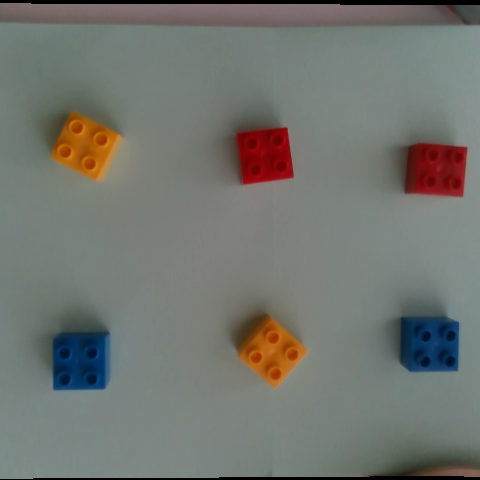
\includegraphics[width=1\textwidth]{Segmentacion por color/colour.png}
	\end{minipage}}
  \hfill	
  \subfloat{
	\begin{minipage}[c][1\width]{0.3\textwidth}
	   \centering
	   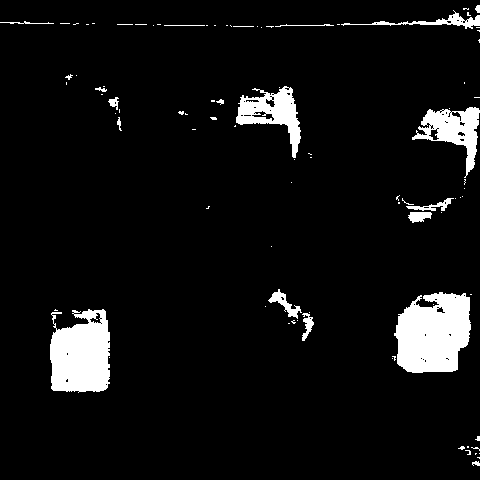
\includegraphics[width=1\textwidth]{Segmentacion por color/error_binario.png}
	\end{minipage}}
  \hfill	
  \subfloat{
	\begin{minipage}[c][1\width]{0.3\textwidth}
	   \centering
	   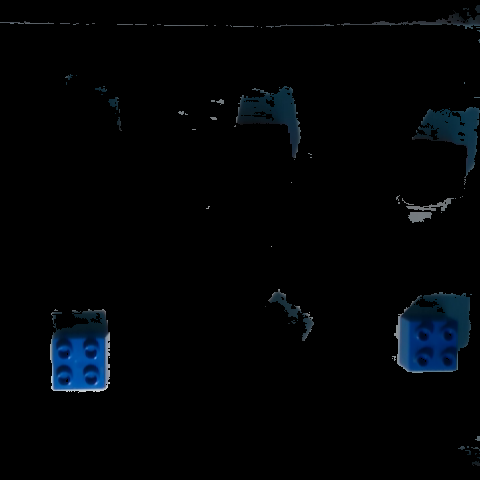
\includegraphics[width=1\textwidth]{Segmentacion por color/error.png}
	\end{minipage}}
\caption{Error por mala calibración del filtrado por color}
\label{fig:colour2}
\vspace{-5pt}
\end{figure}

Para el desarrollo de los filtros por color, se ha usado una herramienta de MATLAB llamada \texttt{colorThresholder}. Con la ayuda de esta herramienta se han creado tres funciones. Una función para cada color la cual devuelve la imagen binaria y la combinación de la imagen original y la imagen binaria.

\begin{figure}[ht]  %Filtrado por color
  \subfloat{
	\begin{minipage}[c][1\width]{0.3\textwidth}
	   \centering
	   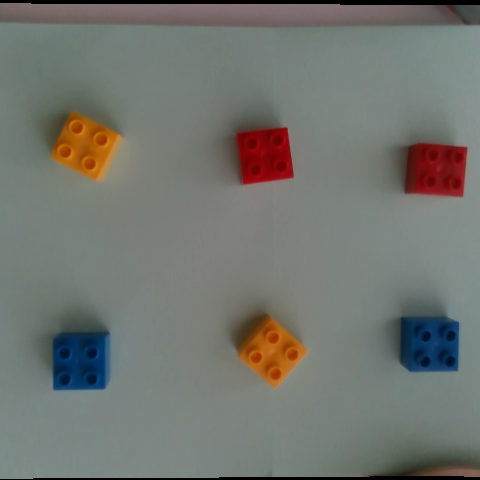
\includegraphics[width=1\textwidth]{Segmentacion por color/colour.png}
	\end{minipage}}
  \hfill	
  \subfloat{
	\begin{minipage}[c][1\width]{0.3\textwidth}
	   \centering
	   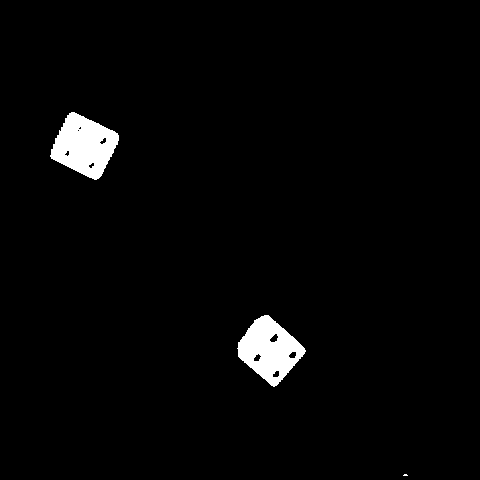
\includegraphics[width=1\textwidth]{Segmentacion por color/yellow_binario.png}
	\end{minipage}}
  \hfill	
  \subfloat{
	\begin{minipage}[c][1\width]{0.3\textwidth}
	   \centering
	   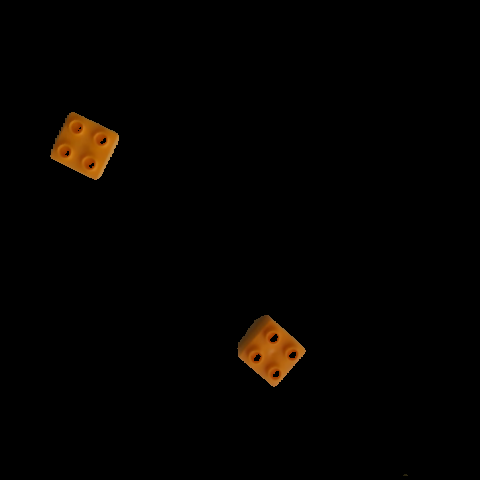
\includegraphics[width=1\textwidth]{Segmentacion por color/yellow.png}
	\end{minipage}}
  
  \medskip
  
  \subfloat{
	\begin{minipage}[c][1\width]{0.3\textwidth}
	   \centering
	   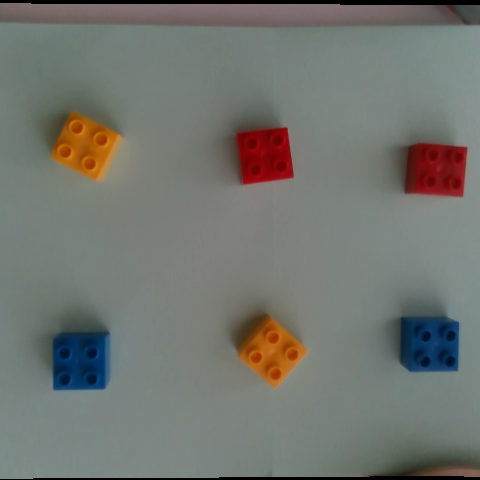
\includegraphics[width=1\textwidth]{Segmentacion por color/colour.png}
	\end{minipage}}
  \hfill	
  \subfloat{
	\begin{minipage}[c][1\width]{0.3\textwidth}
	   \centering
	   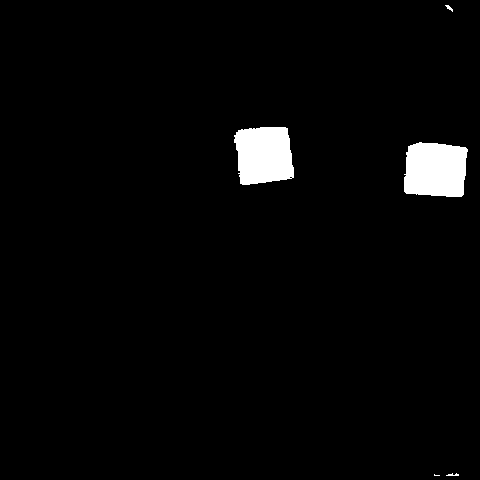
\includegraphics[width=1\textwidth]{Segmentacion por color/red_binario.png}
	\end{minipage}}
  \hfill	
  \subfloat{
	\begin{minipage}[c][1\width]{0.3\textwidth}
	   \centering
	   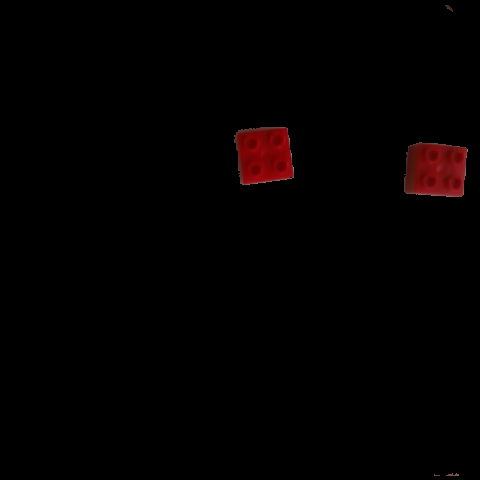
\includegraphics[width=1\textwidth]{Segmentacion por color/red.png}
	\end{minipage}}
	
  \medskip
  
  \subfloat{
	\begin{minipage}[c][1\width]{0.3\textwidth}
	   \centering
	   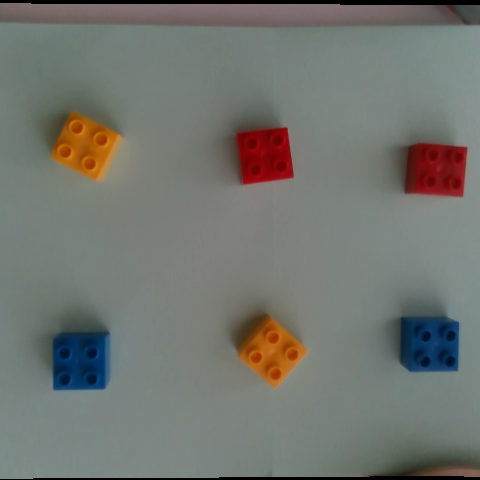
\includegraphics[width=1\textwidth]{Segmentacion por color/colour.png}
	\end{minipage}}
  \hfill	
  \subfloat{
	\begin{minipage}[c][1\width]{0.3\textwidth}
	   \centering
	   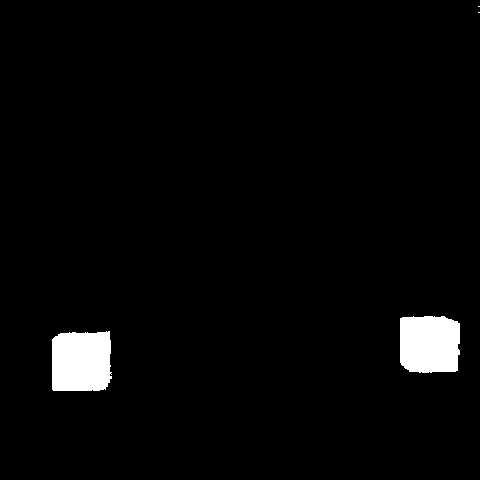
\includegraphics[width=1\textwidth]{Segmentacion por color/blue_binario.png}
	\end{minipage}}
  \hfill	
  \subfloat{
	\begin{minipage}[c][1\width]{0.3\textwidth}
	   \centering
	   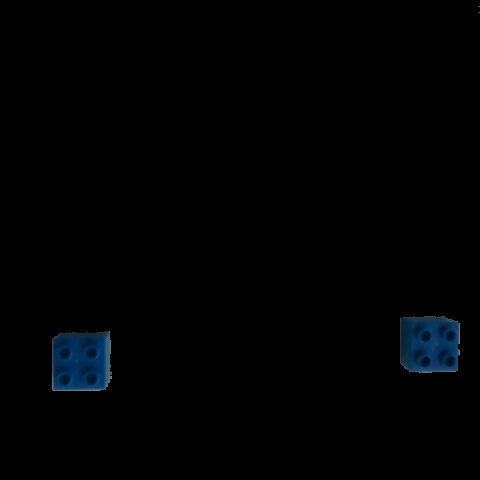
\includegraphics[width=1\textwidth]{Segmentacion por color/blue.png}
	\end{minipage}}
\caption{Filtrado por color}
\label{fig:colour}
\end{figure}

\clearpage
\section{Identificación y mejora de la imagen}
Una vez aplicado el filtro de color se realiza un estudio exhaustivo de las piezas. Este comienza por la separación de las piezas para cada color. Para ello, primero se hace una limpieza de la imagen eliminando los pequeños objetos de la imagen binaria (ruido). A continuación, se emplea la función de MATLAB \texttt{regionprops} que devuelve las propiedades de los objetos encontrados y el número de objetos encontrados. De esta forma, ya sabemos el número de piezas de cada color y de forma aproximada su posición y área.

Desgraciadamente la información extraída con \texttt{regionprops} no es suficientemente precisa. Sobre todo, cuando se tienen varias piezas apiladas ya que con los filtros también se puede haber detectado las piezas inferiores aumentando así el tamaño de la pieza. Por ello es necesario un estudio más exhaustivo analizando cada pieza de forma independiente. Para facilitar el cálculo y la mejor detección de la pieza, se pasan todas las piezas a escala de grises \citep{greyscale}. A continuación, se muestran el proceso de separación de piezas y transformación a escala de grises.

El proceso a seguir para mejorar la precisión de la detección de la pieza consiste en eliminar el borde de la pieza y los elementos pequeños. De esta forma se intenta solo detectar la cara superior del LEGO. Una vez eliminado el borde se vuelve a emplear regionprops para obtener todas las propiedades, pero con una mayor precisión.

Para poder detectar correctamente el borde y eliminarlo de la imagen primero es necesario ajustar y filtrar la imagen. El proceso total de mejora de la imagen y extracción de características consta de cinco pasos:

\begin{enumerate}
\item Se realiza un ajuste de de la intensidad de la imagen en escala de grises. De esta forma se resaltan más los cambios de color/iluminación.

\item Se desea resaltar aún más los detalles de la imagen. Esto se va a llevar a cabo con la ayuda de un filtro de difuminado Gaussiano. Primero se difumina la imagen para ensalzar los rasgos generales y después se le restan estos rasgos a la imagen original. De esta forma se destacan los pequeños detalles.

\item Una vez mejorada la imagen, toca detectar el borde de la pieza. Para ello se va a aplicar el algoritmo de Canny.

\item Al filtrar las imágenes por color también se puede haber incluido las caras laterales de la pieza y las caras laterales de las piezas situadas debajo de la pieza a detectar. Para reducir el efecto que esto puede causar, se ensanchan los bordes de forma que incluyan pequeños detalles que puedan estropear el proceso.

\item El último paso para obtener la cara interna del LEGO consiste en invertir los colores de los bordes obtenidos. De esta forma, solo se conserva la cara interna.
\end{enumerate}


\begin{figure}[p]  %Selección de la pieza
  \subfloat{
	\begin{minipage}[c][1\width]{0.3\textwidth}
	   \centering
	   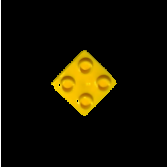
\includegraphics[width=1\textwidth]{Segmentacion por color/amarillo_aux.png}
	\end{minipage}}
  \hfill	
  \subfloat{
	\begin{minipage}[c][1\width]{0.3\textwidth}
	   \centering
	   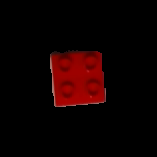
\includegraphics[width=1\textwidth]{Segmentacion por color/red_aux.png}
	\end{minipage}}
  \hfill	
  \subfloat{
	\begin{minipage}[c][1\width]{0.3\textwidth}
	   \centering
	   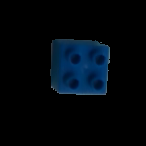
\includegraphics[width=1\textwidth]{Segmentacion por color/blue_aux.png}
	\end{minipage}}
\caption{Segmentación de las piezas a analizar}
\label{fig:mejora1}
\vspace{-5pt}
\end{figure}

\begin{figure}[p]  %Escalado de grises
  \subfloat{
	\begin{minipage}[c][1\width]{0.3\textwidth}
	   \centering
	   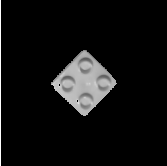
\includegraphics[width=1\textwidth]{Segmentacion por color/amarillo_aux_ad.png}
	\end{minipage}}
  \hfill	
  \subfloat{
	\begin{minipage}[c][1\width]{0.3\textwidth}
	   \centering
	   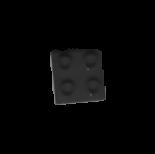
\includegraphics[width=1\textwidth]{Segmentacion por color/red_aux_ad.png}
	\end{minipage}}
  \hfill	
  \subfloat{
	\begin{minipage}[c][1\width]{0.3\textwidth}
	   \centering
	   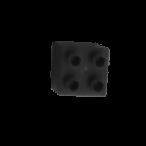
\includegraphics[width=1\textwidth]{Segmentacion por color/blue_aux_ad.png}
	\end{minipage}}
\caption{Escalado a gris de las piezas segmentadas}
\label{fig:mejora2}
\vspace{-5pt}
\end{figure}

\begin{figure}[p]  %Primer paso
  \subfloat{
	\begin{minipage}[c][1\width]{0.3\textwidth}
	   \centering
	   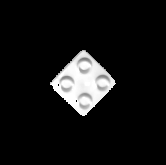
\includegraphics[width=1\textwidth]{Segmentacion por color/amarillo_ad.png}
	\end{minipage}}
  \hfill	
  \subfloat{
	\begin{minipage}[c][1\width]{0.3\textwidth}
	   \centering
	   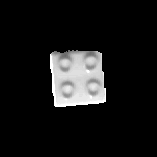
\includegraphics[width=1\textwidth]{Segmentacion por color/red_ad.png}
	\end{minipage}}
  \hfill	
  \subfloat{
	\begin{minipage}[c][1\width]{0.3\textwidth}
	   \centering
	   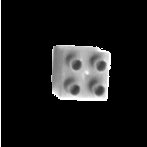
\includegraphics[width=1\textwidth]{Segmentacion por color/blue_ad.png}
	\end{minipage}}
\caption{Primer paso: ajuste de intensidad}
\label{fig:mejora3}
\vspace{-5pt}
\end{figure}

\begin{figure}[p]  %Segundo y tercer paso
  \subfloat{
	\begin{minipage}[c][1\width]{0.3\textwidth}
	   \centering
	   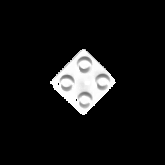
\includegraphics[width=1\textwidth]{Segmentacion por color/amarillo_fin2.png}
	\end{minipage}}
  \hfill	
  \subfloat{
	\begin{minipage}[c][1\width]{0.3\textwidth}
	   \centering
	   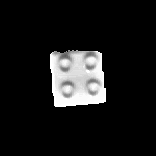
\includegraphics[width=1\textwidth]{Segmentacion por color/red_fin2.png}
	\end{minipage}}
  \hfill	
  \subfloat{
	\begin{minipage}[c][1\width]{0.3\textwidth}
	   \centering
	   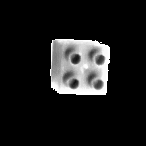
\includegraphics[width=1\textwidth]{Segmentacion por color/blue_fin2.png}
	\end{minipage}}
\caption{Segundo paso: Resalto de pequeños detalles}
\label{fig:mejora4}
\vspace{-5pt}
\end{figure}

\begin{figure}[p]  %Tercer paso
  \subfloat{
	\begin{minipage}[c][1\width]{0.3\textwidth}
	   \centering
	   
\includegraphics[width=1\textwidth]{Segmentacion por color/amarillo_f.png}
	\end{minipage}}
  \hfill	
  \subfloat{
	\begin{minipage}[c][1\width]{0.3\textwidth}
	   \centering
	   
\includegraphics[width=1\textwidth]{Segmentacion por color/red_f.png}
	\end{minipage}}
  \hfill	
  \subfloat{
	\begin{minipage}[c][1\width]{0.3\textwidth}
	   \centering
	   
\includegraphics[width=1\textwidth]{Segmentacion por color/blue_f.png}
	\end{minipage}}
\caption{Tercer paso: aplicación del algoritmo de Canny}
\label{fig:mejora5}
\vspace{-5pt}
\end{figure}

\begin{figure}[p]	 %Cuarto paso
  \subfloat{
	\begin{minipage}[c][1\width]{0.3\textwidth}
	   \centering
	   
\includegraphics[width=1\textwidth]{Segmentacion por color/amarillo_d.png}
	\end{minipage}}
  \hfill	
  \subfloat{
	\begin{minipage}[c][1\width]{0.3\textwidth}
	   \centering
	   
\includegraphics[width=1\textwidth]{Segmentacion por color/red_c.png}
	\end{minipage}}
  \hfill	
  \subfloat{
	\begin{minipage}[c][1\width]{0.3\textwidth}
	   \centering
	   
\includegraphics[width=1\textwidth]{Segmentacion por color/blue_c.png}
	\end{minipage}}
\caption{Cuarto paso: dilatación y contracción de los bordes}
\label{fig:mejora6}
\vspace{-5pt}
\end{figure}

\begin{figure}[p]  %Quinto paso
  \subfloat{
	\begin{minipage}[c][1\width]{0.3\textwidth}
	   \centering
	   
\includegraphics[width=1\textwidth]{Segmentacion por color/amarillo_b.png}
	\end{minipage}}
  \hfill	
  \subfloat{
	\begin{minipage}[c][1\width]{0.3\textwidth}
	   \centering
	   
\includegraphics[width=1\textwidth]{Segmentacion por color/red_b.png}
	\end{minipage}}
  \hfill	
  \subfloat{
	\begin{minipage}[c][1\width]{0.3\textwidth}
	   \centering
	   
\includegraphics[width=1\textwidth]{Segmentacion por color/blue_b.png}
	\end{minipage}}
\caption{Quinto paso: Inversión de los colores de la pieza}
\label{fig:mejora7}
\vspace{-5pt}
\end{figure}

\clearpage
\section{Extracción de características}
El último paso para la obtención de las características de la pieza se vuelve a emplear la función \texttt{regionprops} de MATLAB. con cada una de las piezas identificadas. Al trabajarse de forma individual con cada pieza y como estas has sido mejoradas, la precisión es bastante elevada y se puede obtener de forma bastante precisa el centroide de cada pieza.

\section{Resultados}
\label{sec:color resultados}
Para comprobar la eficacia de la segmentación por color, se ha desarrollado un \textit{script} con la ayuda de MATLAB para determinar su capacidad de para identificar piezas y la precisión con las que la detecta. En este \textit{script} se han analizado 74 imágenes con más de 380 piezas de LEGO. Y con el fin de obtener un análisis riguroso y que refleje la capacidad de este método ante diversas condiciones, se han seleccionado fotos con múltiples ángulos y escenas. A continuación, se muestra algunas de las imágenes usadas para la evaluación:

\begin{figure}[ht]  %Entrenamiento segmentación
	\centering
	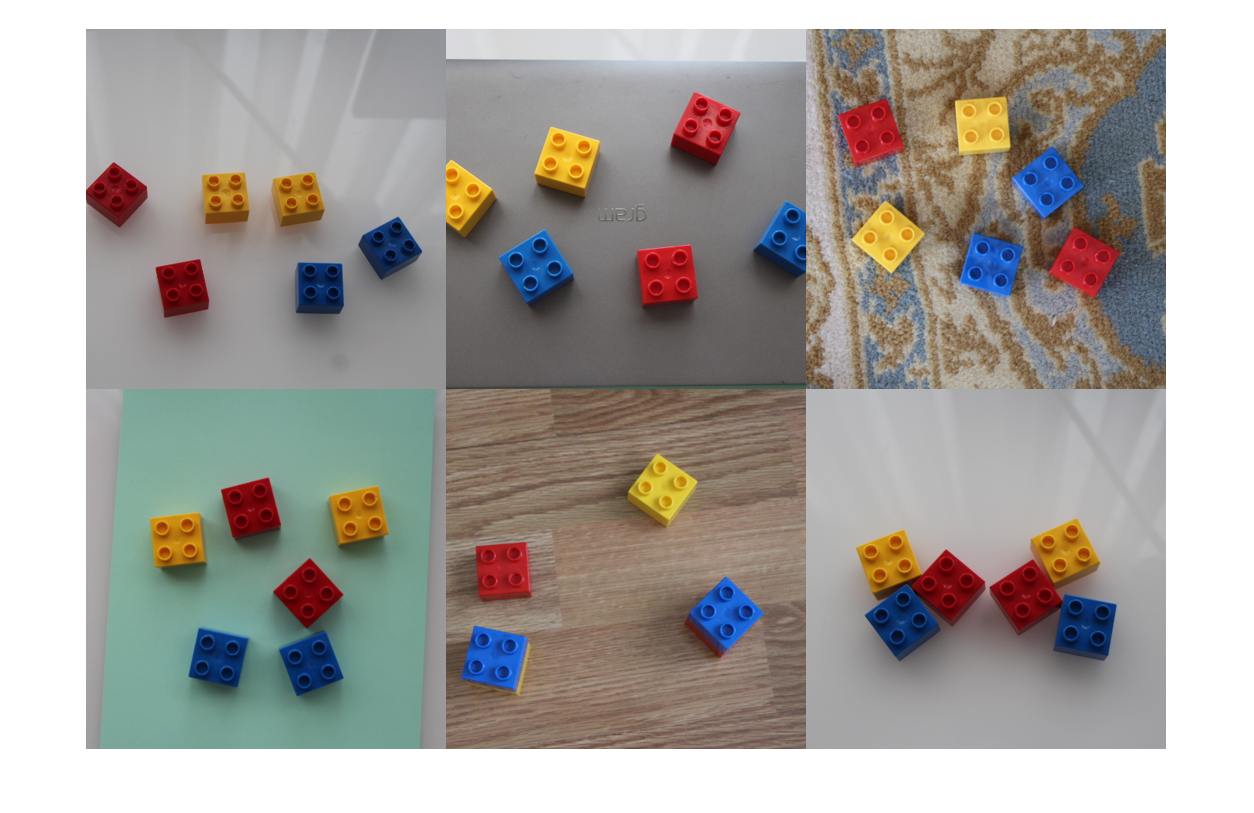
\includegraphics[width=0.8\textwidth]{Segmentacion por color/entrenamiento.png}
	\caption{Muestra de imágenes para la evaluación del proceso de segmentación}
	\label{fig:entrenamiento}
\end{figure}

Con la ayuda del \textit{script} se han podido obtener cuatro parámetros que permiten evaluar los resultados. En primer lugar, se ha obtenido la tasa de fallos y el número de falsos positivos por imagen para cada una de las clases. Y a continuación se ha evaluado la precisión de las piezas encontradas y la exhaustividad, que es la relación entre verdaderos positivos y la suma de verdaderos positivos y falsos negativos.

Tras analizar los resultados se ha llegado a las siguientes conclusiones:
\begin{itemize}
\item Amarillo: Del total de piezas, estas han sido las que mejor han sido detectadas. Presentan una precisión muy elevada y una tasa de fallos muy pequeña. Las formas de las gráficas se deben a que este método apenas ha tenido falsos positivos y cuando estos han ocurrido estaban muy controlados. Es por ello que la gráfica es tan brusca y con tan pocos puntos.
\item Rojo: La tasa de fallos es bastante superior respecto al amarillo y la precisión también baja bastante. Esto de nuevo se debe al filtro de color. En los resultados se han dado numerosos falsos positivos y en numerosas ocasiones ha habido piezas rojas que no se han detectado. Esto explica los valores de exhaustividad obtenidos y el porqué de que aunque la exhaustividad no sea muy elevado, la precisión es muy baja.
\item Azul: El azul sufre de los mismos problemas que el rojo. Hay demasiados falsos positivos y múltiples situaciones en las que a pesar de haber falsos positivos, no se han detectado las piezas azules.
\end{itemize}

\begin{figure}[ht]  %Estudio Amarillo
  \subfloat{
	\begin{minipage}[c][1\width]{0.49\textwidth}
	   \centering
	   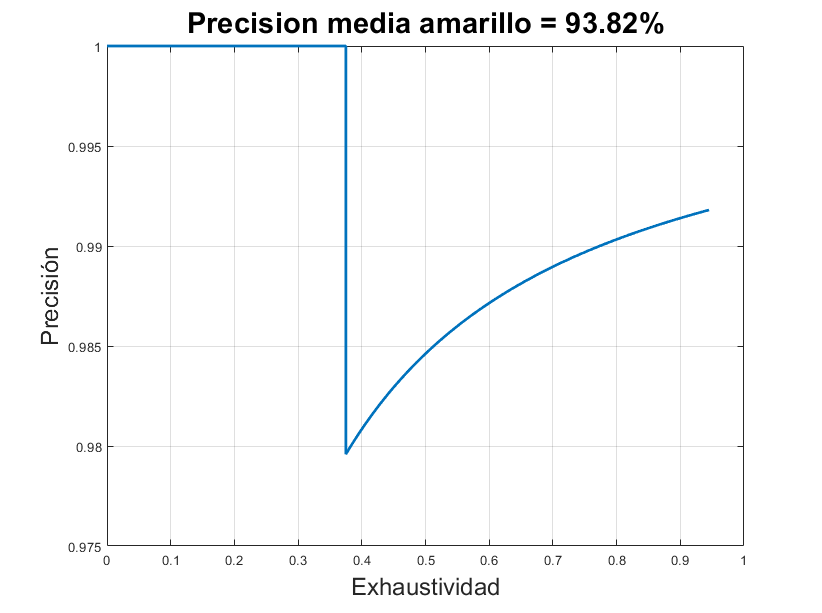
\includegraphics[width=1\textwidth]{Segmentacion por color/precision_yellow.png}
	\end{minipage}}
  \hfill	
  \subfloat{
	\begin{minipage}[c][1\width]{0.49\textwidth}
	   \centering
	   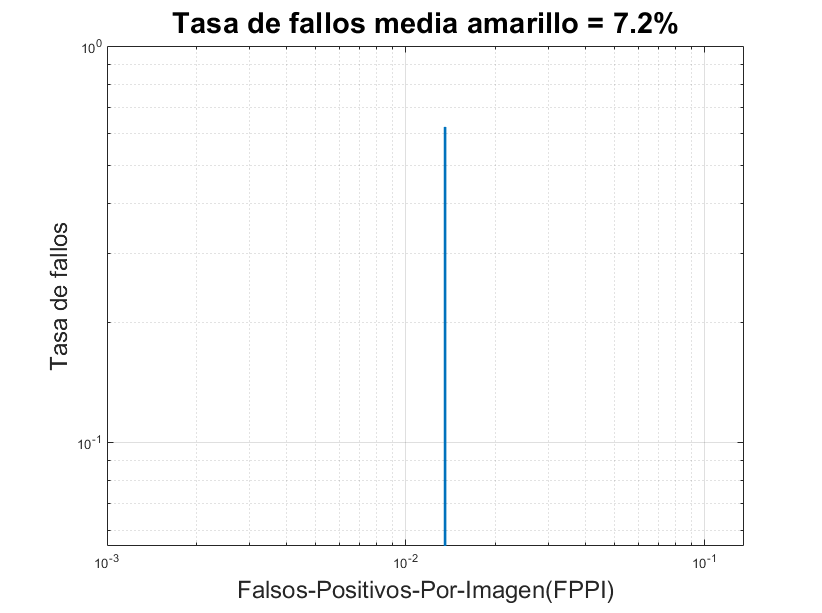
\includegraphics[width=1\textwidth]{Segmentacion por color/miss_yellow.png}
	\end{minipage}}
\caption{Estudio de la segmentación por color al detectar piezas amarillas}
\label{fig:yellow colour}
\vspace{-5pt}
\end{figure}

\begin{figure}[ht]  %Estudio Rojo
  \subfloat{
	\begin{minipage}[c][1\width]{0.49\textwidth}
	   \centering
	   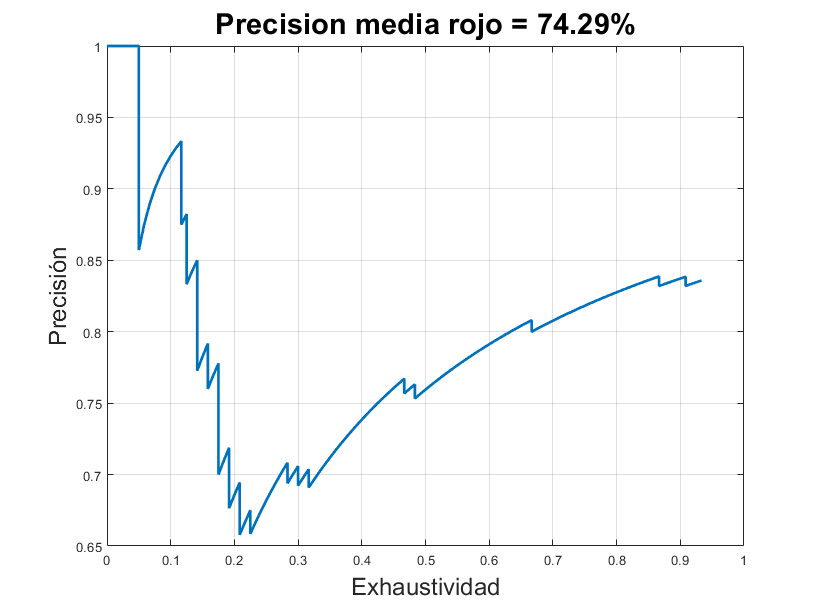
\includegraphics[width=1\textwidth]{Segmentacion por color/precision_red.png}
	\end{minipage}}
  \hfill	
  \subfloat{
	\begin{minipage}[c][1\width]{0.49\textwidth}
	   \centering
	   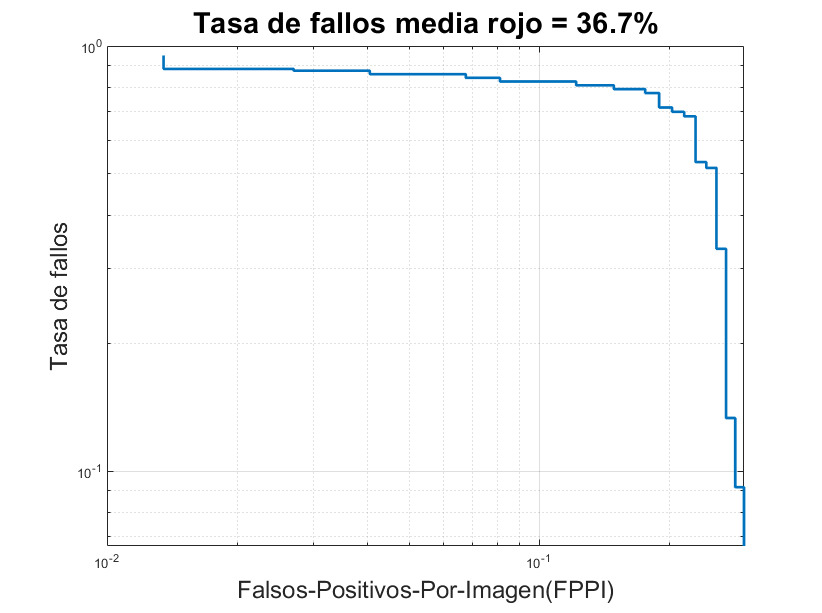
\includegraphics[width=1\textwidth]{Segmentacion por color/miss_red.png}
	\end{minipage}}
\caption{Estudio de la segmentación por color al detectar piezas rojas}
\label{fig:red colour}
\vspace{-5pt}
\end{figure}

\begin{figure}[ht]  %Estudio Azul
  \subfloat{
	\begin{minipage}[c][1\width]{0.49\textwidth}
	   \centering
	   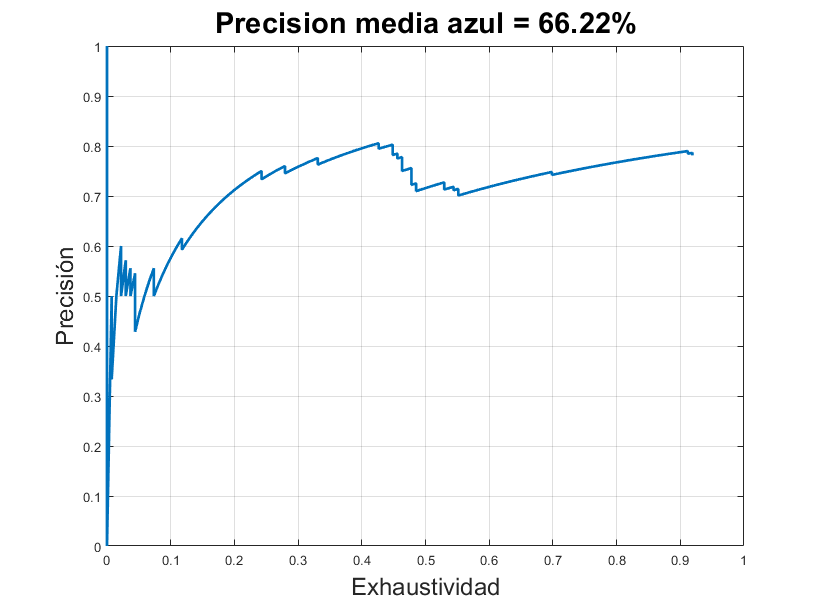
\includegraphics[width=1\textwidth]{Segmentacion por color/precision_blue.png}
	\end{minipage}}
  \hfill	
  \subfloat{
	\begin{minipage}[c][1\width]{0.49\textwidth}
	   \centering
	   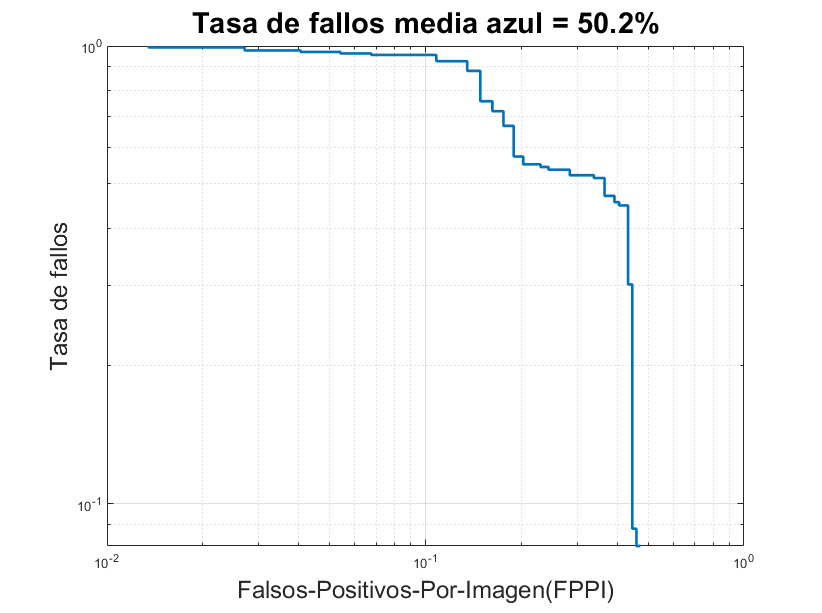
\includegraphics[width=1\textwidth]{Segmentacion por color/miss_blue.png}
	\end{minipage}}
\caption{Estudio de la segmentación por color al detectar piezas azules}
\label{fig:blue colour}
\vspace{-5pt}
\end{figure}

\begin{figure}[ht]  %Entrenamiento segmentación
	\centering
	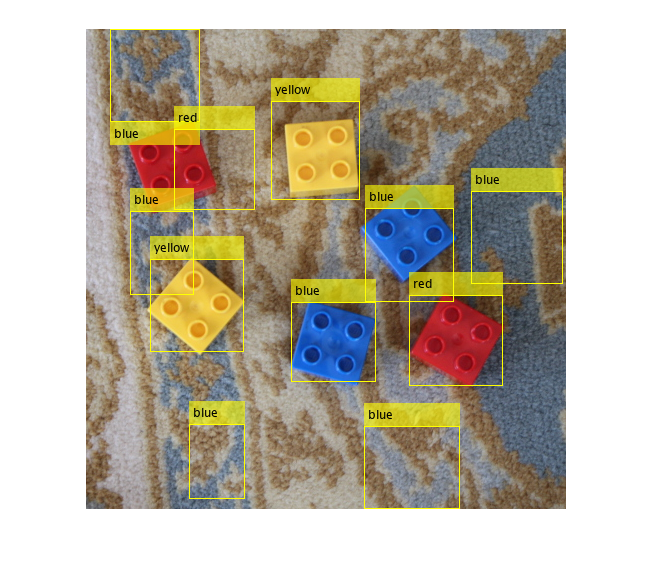
\includegraphics[width=0.8\textwidth]{Segmentacion por color/error_evaluacion.png}
	\caption{Error en la evaluación de segmentación por color}
	\label{fig:error entrenamiento}
\end{figure}
